% Created by tikzDevice version 0.10.1 on 2017-12-03 20:41:30
% !TEX encoding = UTF-8 Unicode
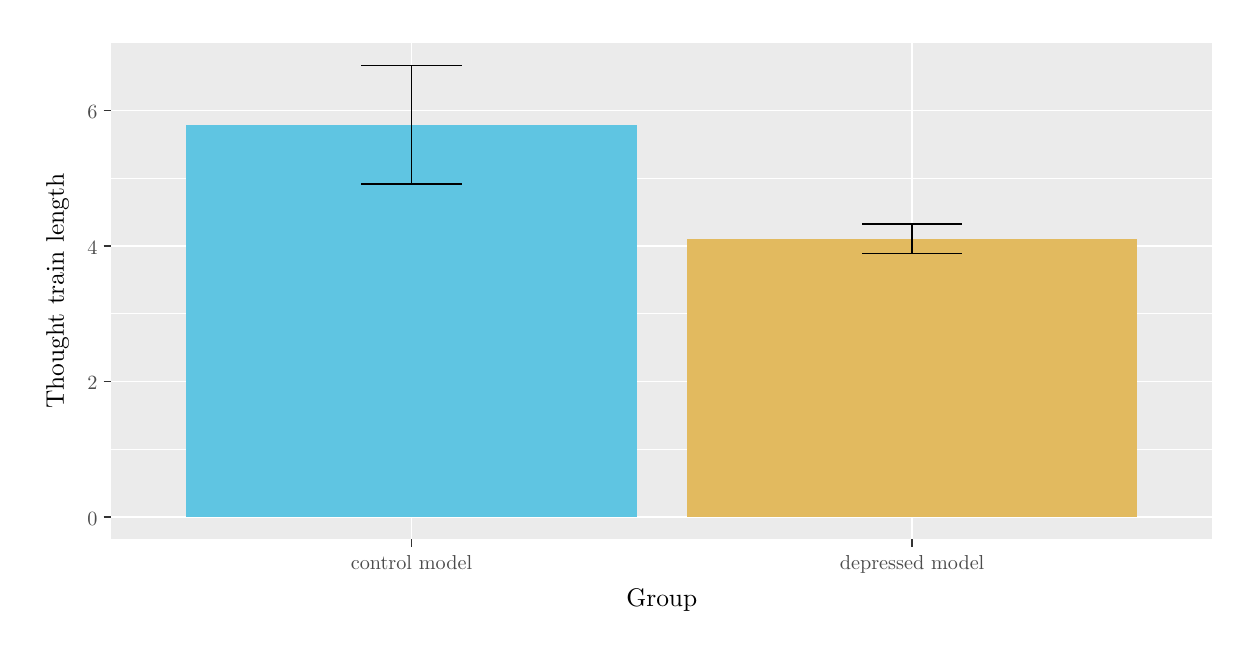
\begin{tikzpicture}[x=1pt,y=1pt]
\definecolor{fillColor}{RGB}{255,255,255}
\path[use as bounding box,fill=fillColor,fill opacity=0.00] (0,0) rectangle (433.62,216.81);
\begin{scope}
\path[clip] (  0.00,  0.00) rectangle (433.62,216.81);
\definecolor{drawColor}{RGB}{255,255,255}
\definecolor{fillColor}{RGB}{255,255,255}

\path[draw=drawColor,line width= 0.6pt,line join=round,line cap=round,fill=fillColor] (  0.00,  0.00) rectangle (433.62,216.81);
\end{scope}
\begin{scope}
\path[clip] ( 30.17, 31.92) rectangle (428.12,211.31);
\definecolor{fillColor}{gray}{0.92}

\path[fill=fillColor] ( 30.17, 31.92) rectangle (428.12,211.31);
\definecolor{drawColor}{RGB}{255,255,255}

\path[draw=drawColor,line width= 0.3pt,line join=round] ( 30.17, 64.54) --
	(428.12, 64.54);

\path[draw=drawColor,line width= 0.3pt,line join=round] ( 30.17,113.48) --
	(428.12,113.48);

\path[draw=drawColor,line width= 0.3pt,line join=round] ( 30.17,162.42) --
	(428.12,162.42);

\path[draw=drawColor,line width= 0.6pt,line join=round] ( 30.17, 40.07) --
	(428.12, 40.07);

\path[draw=drawColor,line width= 0.6pt,line join=round] ( 30.17, 89.01) --
	(428.12, 89.01);

\path[draw=drawColor,line width= 0.6pt,line join=round] ( 30.17,137.95) --
	(428.12,137.95);

\path[draw=drawColor,line width= 0.6pt,line join=round] ( 30.17,186.89) --
	(428.12,186.89);

\path[draw=drawColor,line width= 0.6pt,line join=round] (138.70, 31.92) --
	(138.70,211.31);

\path[draw=drawColor,line width= 0.6pt,line join=round] (319.59, 31.92) --
	(319.59,211.31);
\definecolor{fillColor}{RGB}{95,197,226}

\path[fill=fillColor] ( 57.30, 40.07) rectangle (220.10,181.77);
\definecolor{fillColor}{RGB}{226,186,95}

\path[fill=fillColor] (238.19, 40.07) rectangle (400.99,140.48);
\definecolor{drawColor}{RGB}{0,0,0}

\path[draw=drawColor,line width= 0.6pt,line join=round] (120.61,203.16) --
	(156.79,203.16);

\path[draw=drawColor,line width= 0.6pt,line join=round] (138.70,203.16) --
	(138.70,160.38);

\path[draw=drawColor,line width= 0.6pt,line join=round] (120.61,160.38) --
	(156.79,160.38);

\path[draw=drawColor,line width= 0.6pt,line join=round] (301.50,145.81) --
	(337.68,145.81);

\path[draw=drawColor,line width= 0.6pt,line join=round] (319.59,145.81) --
	(319.59,135.15);

\path[draw=drawColor,line width= 0.6pt,line join=round] (301.50,135.15) --
	(337.68,135.15);
\end{scope}
\begin{scope}
\path[clip] (  0.00,  0.00) rectangle (433.62,216.81);
\definecolor{drawColor}{gray}{0.30}

\node[text=drawColor,anchor=base east,inner sep=0pt, outer sep=0pt, scale=  0.73] at ( 25.22, 37.04) {0};

\node[text=drawColor,anchor=base east,inner sep=0pt, outer sep=0pt, scale=  0.73] at ( 25.22, 85.98) {2};

\node[text=drawColor,anchor=base east,inner sep=0pt, outer sep=0pt, scale=  0.73] at ( 25.22,134.92) {4};

\node[text=drawColor,anchor=base east,inner sep=0pt, outer sep=0pt, scale=  0.73] at ( 25.22,183.86) {6};
\end{scope}
\begin{scope}
\path[clip] (  0.00,  0.00) rectangle (433.62,216.81);
\definecolor{drawColor}{gray}{0.20}

\path[draw=drawColor,line width= 0.6pt,line join=round] ( 27.42, 40.07) --
	( 30.17, 40.07);

\path[draw=drawColor,line width= 0.6pt,line join=round] ( 27.42, 89.01) --
	( 30.17, 89.01);

\path[draw=drawColor,line width= 0.6pt,line join=round] ( 27.42,137.95) --
	( 30.17,137.95);

\path[draw=drawColor,line width= 0.6pt,line join=round] ( 27.42,186.89) --
	( 30.17,186.89);
\end{scope}
\begin{scope}
\path[clip] (  0.00,  0.00) rectangle (433.62,216.81);
\definecolor{drawColor}{gray}{0.20}

\path[draw=drawColor,line width= 0.6pt,line join=round] (138.70, 29.17) --
	(138.70, 31.92);

\path[draw=drawColor,line width= 0.6pt,line join=round] (319.59, 29.17) --
	(319.59, 31.92);
\end{scope}
\begin{scope}
\path[clip] (  0.00,  0.00) rectangle (433.62,216.81);
\definecolor{drawColor}{gray}{0.30}

\node[text=drawColor,anchor=base,inner sep=0pt, outer sep=0pt, scale=  0.73] at (138.70, 20.91) {control model};

\node[text=drawColor,anchor=base,inner sep=0pt, outer sep=0pt, scale=  0.73] at (319.59, 20.91) {depressed model};
\end{scope}
\begin{scope}
\path[clip] (  0.00,  0.00) rectangle (433.62,216.81);
\definecolor{drawColor}{RGB}{0,0,0}

\node[text=drawColor,anchor=base,inner sep=0pt, outer sep=0pt, scale=  0.92] at (229.14,  7.83) {Group};
\end{scope}
\begin{scope}
\path[clip] (  0.00,  0.00) rectangle (433.62,216.81);
\definecolor{drawColor}{RGB}{0,0,0}

\node[text=drawColor,rotate= 90.00,anchor=base,inner sep=0pt, outer sep=0pt, scale=  0.92] at ( 13.08,121.61) {Thought train length};
\end{scope}
\end{tikzpicture}
